\documentclass[11pt]{article}
\usepackage{amsmath,amssymb,amsthm}
\usepackage{algorithm}
\usepackage{algorithmic}
\usepackage{graphicx}
\usepackage{booktabs}
\usepackage{hyperref}
\usepackage{natbib}
\usepackage{xcolor}
\usepackage{enumitem}

% Theorem environments
\newtheorem{theorem}{Theorem}[section]
\newtheorem{lemma}[theorem]{Lemma}
\newtheorem{proposition}[theorem]{Proposition}
\newtheorem{corollary}[theorem]{Corollary}
\newtheorem{definition}[theorem]{Definition}

% Notation shortcuts
\newcommand{\R}{\mathbb{R}}
\newcommand{\norm}[1]{\|#1\|}

% Title and authors
\title{Rank-Preserving Calibration for Multiclass Classification}

\author{
Gaurav Sood\thanks{Corresponding author: contact@gsood.com}
}

\date{}

\begin{document}

\maketitle

\begin{abstract}
Post-hoc calibration for multiclass classifiers faces two competing goals: match known class totals (label marginals) and preserve the within-class ranking of instances induced by the original model. Classical prior-correction methods and per-class logit shifts match totals but can scramble rankings via instance-specific softmax renormalization; popular multiclass calibrators (temperature, matrix/vector scaling, Dirichlet) reduce calibration error but do not enforce rank preservation. We formulate calibration as Euclidean projection onto the intersection of a row-simplex set and a columnwise isotonic-plus-sum set, where isotonic order within each class is defined by the model's pre-calibration scores. We provide a Dykstra alternating-projection solver and an ADMM splitting; the column subproblem admits an exact one-pass PAV solution followed by a scalar shift to satisfy the column sum constraint. Nearly-isotonic variants trade small, controlled rank violations for calibration gains. Experiments on neural and tabular benchmarks show that the method matches target totals while preserving within-class orderings and maintaining competitive ECE/Brier scores. Our Python implementation is open source.\footnote{\url{https://github.com/finite-sample/rank_preserving_calibration}}
\end{abstract}

\section{Introduction}

Calibration of probabilistic classifiers is essential for decision-making where predicted probabilities should reflect empirical frequencies. In many applications, from health to finance to survey weighting, practitioners must both adjust predictions to match known class totals and maintain the model's within-class discrimination, the relative ordering of instances within each class.

In the multiclass setting ($J \ge 3$), naive per-class logit shifts (or label-prior corrections) can change instance orderings within a class because the softmax renormalization term varies by instance. Standard multiclass calibrators such as temperature scaling \citep{guo2017} and Dirichlet calibration \citep{kull2019} improve calibration but do not guarantee order preservation. Label-shift and prior-correction methods \citep{saerens2002,lipton2018} match marginals but can induce the same ranking problem.

\subsection{The Rank-Scrambling Problem}
Given original probabilities $p_{ij}$ and per-class multiplicative weights $w_j$, the adjusted probabilities
\[
q_{ij} \;=\; \frac{w_j p_{ij}}{\sum_{k=1}^J w_k p_{ik}}
\]
depend on the instance-specific denominator. Hence $p_{i_1 j} > p_{i_2 j}$ need not imply $q_{i_1 j} > q_{i_2 j}$.

\paragraph{Worked example (3 classes, two instances).}
\[
p_{1,\cdot}=(0.51,\,0.48,\,0.01),\quad p_{2,\cdot}=(0.49,\,0.02,\,0.49),\quad w=(1,\,100,\,1).
\]
Then $q_{11}=0.51/(0.51+48+0.01)\approx 0.0105$ while $q_{21}=0.49/(0.49+2+0.49)\approx 0.1644$, reversing the original class-$1$ order.

\subsection{Our Approach}

We project the original probability matrix onto the intersection of the row-simplex and per-column isotonic-plus-sum sets, where isotonic order is the total preorder induced by the original scores for that class. This formulation guarantees rank preservation and exact total matching by construction. We develop two solvers: a Dykstra alternating-projection method \citep{dykstra1983} and an ADMM splitting. The column projection in both cases is solved exactly by a single PAV pass followed by a scalar shift to match the target column sum. We also provide nearly-isotonic variants with $\epsilon$-slack and hinge-penalty relaxations that allow practitioners to tune the calibration-discrimination tradeoff. Across neural and tabular classifiers, the method matches targets while preserving within-class weak orders and maintaining competitive calibration metrics.

\section{Related Work}

\paragraph{Label/prior shift and matching marginals.}
When deployment priors differ from training priors, the EM update of \citet{saerens2002} and black-box shift estimation \citep{lipton2018} adjust predicted posteriors to match new class totals without refitting. These methods are effective for marginals but apply instance-specific renormalization that can reverse within-class orderings when $J\!\ge\!3$.

\paragraph{Multiclass calibration.}
Temperature scaling and class-wise linear maps (vector/matrix scaling) \citep{guo2017} and Dirichlet calibration \citep{kull2019} are widely used but do not enforce within-class ranking constraints. Recent work explores ranking-aware criteria \citep{ma2021metacal} and normalization-aware isotonic approaches for multiclass settings \citep{arad2025}; neither simultaneously enforces rank preservation and matches given class totals.

\section{Problem Formulation}

Let $P \in \R^{N\times J}_+$ be the matrix of predicted probabilities, with rows on the probability simplex. We seek $Q \in \R^{N\times J}_+$ satisfying three constraints: each row sums to one ($\sum_{j=1}^J Q_{ij}=1$ for all $i$, $Q_{ij}\ge 0$); each column sums to its target ($\sum_{i=1}^N Q_{ij}=T_j$); and each column is isotonic in the order defined by the original scores ($Q_{\cdot j}$ is nondecreasing when rows are sorted by $P_{\cdot j}$, with ties respected). We solve the projection
\begin{equation}
\min_{Q} \;\frac{1}{2}\norm{Q-P}_F^2 \quad \text{s.t.}\quad Q \in S_{\text{row}} \cap I_{\text{cols}}.
\label{eq:main_problem}
\end{equation}

The intersection is nonempty whenever $\sum_{j=1}^J T_j=N$ and $0\le T_j\le N$ for all $j$: the constant-column matrix $Q_{ij}=T_j/N$ lies on the row simplex, matches the column totals, and is isotone (constant) in each column.

\section{Algorithms}

\subsection{Dykstra's Alternating Projection Algorithm}

\begin{algorithm}
\caption{Dykstra's method for rank-preserving calibration}
\label{alg:dykstra}
\begin{algorithmic}[1]
\REQUIRE $P \in \R^{N \times J}$, targets $T \in \R^J$, tolerance $\varepsilon$, $\text{max\_iters}$
\STATE Initialize: $Q^{(0)} = P$, $U^{(0)} = 0$, $V^{(0)} = 0$
\FOR{$k = 1$ to $\text{max\_iters}$}
    \STATE $Y^{(k)} = Q^{(k-1)} + U^{(k-1)}$ \hfill (add correction)
    \STATE $Z^{(k)} = \Pi_{\text{row}}(Y^{(k)})$ \hfill (project each row onto the simplex)
    \STATE $U^{(k)} = Y^{(k)} - Z^{(k)}$ \hfill (update correction)
    \STATE $W^{(k)} = Z^{(k)} + V^{(k-1)}$ \hfill (add correction)
    \STATE $Q^{(k)} = \Pi_{\text{iso,sum}}(W^{(k)}, T)$ \hfill (per-column isotone + fixed sum)
    \STATE $V^{(k)} = W^{(k)} - Q^{(k)}$ \hfill (update correction)
    \IF{$\norm{Q^{(k)} - Q^{(k-1)}}_F / \max(1,\norm{Q^{(k-1)}}_F) < \varepsilon$}
        \STATE \textbf{break}
    \ENDIF
\ENDFOR
\RETURN $Q^{(k)}$
\end{algorithmic}
\end{algorithm}

For the row projection $\Pi_{\text{row}}$, we use a fast probability-simplex projection per row with $O(J\log J)$ time via sorting \citep{duchi2008} or Condat's variant \citep{condat2016}.

\subsection{Exact Column Projection: Isotone + Sum Constraint}
For each column $j$, let $w \in \R^N$ be the current column vector arranged in the fixed order that sorts $P_{\cdot j}$ once and for all (stable, ties respected). We seek
\[
\min_{x\in\R^N} \tfrac12\|x-w\|_2^2 \quad \text{s.t.}\quad x_1 \le \cdots \le x_N,\;\; \sum_{i=1}^N x_i = T_j.
\]

\begin{algorithm}
\caption{Column projection $\Pi_{\text{iso,sum}}$ (single PAV + scalar shift)}
\label{alg:colproj}
\begin{algorithmic}[1]
\REQUIRE Column $w\in\R^N$ in fixed score order, target sum $T$
\STATE $y \leftarrow \mathrm{PAV}(w)$
\STATE $c \leftarrow (T - \sum_i y_i)/N$
\STATE \textbf{return} $y + c\cdot \mathbf{1}$
\end{algorithmic}
\end{algorithm}

\begin{lemma}[Isotonic projection with sum constraint]
\label{lem:iso_sum}
Let $C = \{x \in \mathbb{R}^N : x_1 \le \cdots \le x_N\}$ be the isotone cone and $H = \{x : \mathbf{1}^\top x = T\}$ be the sum-constraint hyperplane. If $y = \Pi_C(w)$ denotes the isotonic projection of $w$, then
\[
\Pi_{C \cap H}(w) = y + \frac{T - \mathbf{1}^\top y}{N} \mathbf{1}.
\]
\end{lemma}

\begin{proof}
The isotone cone $C$ is translation-invariant along $\mathbf{1}$: for any $\lambda \in \R$, $x \in C$ if and only if $x + \lambda \mathbf{1} \in C$, so $\Pi_C(w - \lambda \mathbf{1}) = \Pi_C(w) - \lambda \mathbf{1}$. The Lagrangian for the sum-constrained projection
\[
\min_{x \in C} \frac{1}{2}\|x - w\|_2^2 \quad \text{s.t.}\quad \mathbf{1}^\top x = T
\]
introduces a single scalar multiplier $\mu$. The optimality conditions yield $x^\star = y + \mu \mathbf{1}$ where $y = \Pi_C(w)$. The constraint $\mathbf{1}^\top x^\star = T$ gives $\mu = (T - \mathbf{1}^\top y)/N$.
\end{proof}

Nonnegativity is not enforced in this subproblem; it is handled by the subsequent row-simplex projection.

\paragraph{Complexity.}
Per Dykstra iteration: row projections cost $O(NJ\log J)$; column projections are $O(NJ)$ given pre-sorted order. The orders per column are computed once upfront in $O(JN\log N)$.

\subsection{ADMM Formulation}
Introduce $Q=R=S$, with $R\in S_{\text{row}}$ and $S\in I_{\text{cols}}$:
\[
\min_{Q,R,S}\;\frac{1}{2}\norm{Q-P}_F^2\quad\text{s.t.}\;R\in S_{\text{row}},\;S\in I_{\text{cols}},\;Q=R=S.
\]
Standard ADMM updates apply \citep{boyd2011}. The $R$-update is the row-simplex projection; the $S$-update is Algorithm~\ref{alg:colproj}. Warm-starts reuse PAV block structure and previous shifts.

\section{Nearly Isotonic Variants}

\paragraph{Epsilon-slack constraints.}
Replace $x_{i+1}\ge x_i$ with $x_{i+1}\ge x_i-\epsilon$. Let $\tilde x_i = x_i + i\epsilon$. Then $\tilde x$ is standard isotone, and the sum constraint becomes $\sum_i \tilde x_i = T + \epsilon\sum_i i$. Apply Algorithm~\ref{alg:colproj} to $\tilde w$ with target $\tilde T$, then recover $x_i=\tilde x_i - i\epsilon$.

\paragraph{Hinge-penalty approach.}
Add $\lambda\sum_i \max(0, x_i - x_{i+1})$ to the objective. The proximal step can be implemented via splitting: a standard isotonic projection substep plus a shrinkage on violations. We provide a practical solver in the package documentation.

\subsection{The Fundamental Tradeoff}
\label{sec:tradeoff}

Without rank constraints, the natural KL-divergence projection onto the row-simplex constraint with exact column totals has the closed-form solution
\[
q_{ij} = \frac{p_{ij} b_j}{\sum_k p_{ik} b_k},
\]
where $b_j$ are multiplicative weights chosen to satisfy $\sum_i q_{ij} = T_j$. This is the classical multiplicative reweighting form used in label-shift correction \citep{saerens2002,lipton2018}. As the rank-scrambling example in Section~1.1 demonstrates, this exact reweighting can reverse within-class orderings because the instance-specific denominator $\sum_k p_{ik} b_k$ varies by instance, and in multiclass settings this variation can overwhelm the numerator's ordering.

One cannot in general simultaneously achieve the KL-optimal adjustment matching target priors, exact column-sum matching, and exact rank preservation. Our strict Euclidean projection \eqref{eq:main_problem} sacrifices KL-optimality to guarantee total matching and rank preservation. The nearly-isotonic variants allow controlled rank violations to move closer to the KL-optimal solution when small violations are acceptable. We quantify this tradeoff empirically below.

\section{Theoretical Notes}

\paragraph{Convergence.}
For closed convex sets, Dykstra's method converges to the Euclidean projection onto the intersection \citep{bauschke1994}. Rates depend on geometry: polyhedral regularity can yield linear or finite convergence in special cases. We report iteration counts and primal residuals in experiments. ADMM convergence is standard for strongly convex objectives with closed convex constraints \citep{boyd2011,tibshirani2017}.

\paragraph{Rank preservation.}
Because column isotonicity is enforced in the fixed order induced by $P_{\cdot j}$ with stable ties, the calibrated $Q_{\cdot j}$ preserves the original weak order (ties may remain ties).

\section{KL-Divergence Calibration}

The preceding sections focused on Euclidean projection. We now develop a unified Bregman framework that encompasses both Euclidean and KL-divergence calibration, connecting to classical matrix scaling and IPF.

% kl_theory.tex
% Theory section for KL-divergence rank-preserving calibration
% To be included in the follow-up paper

%----------------------------------------------------------------------
% BREGMAN KKT UMBRELLA THEOREM
%----------------------------------------------------------------------

\subsection{Bregman Umbrella Framework}

We present a unified framework for rank-preserving calibration using Bregman divergences,
which includes both Euclidean (squared loss) and KL (relative entropy) as special cases.

Let $D_\phi(Q,R) = \sum_{i,j} \left[\phi(Q_{ij}) - \phi(R_{ij}) - \nabla\phi(R_{ij})(Q_{ij} - R_{ij})\right]$
denote the Bregman divergence generated by a strictly convex function $\phi$.

\begin{theorem}[Bregman KKT Umbrella]
\label{thm:bregman-kkt}
Consider the penalized rank-preserving calibration problem:
\begin{equation}
\min_{Q \in \mathcal{C}(T)} D_\phi(Q, R) + \lambda V_A(Q)
\label{eq:bregman-problem}
\end{equation}
where $\mathcal{C}(T) = \{Q : Q \mathbf{1} = \mathbf{1}, \, Q^\top \mathbf{1} = T, \, Q \geq 0\}$
is the transportation polytope with row-simplex and column-sum constraints,
and $V_A(Q) = \sum_{j=1}^J \sum_{r=1}^{N-1} \omega_{jr} [(D S_j Q_{\cdot j})_r]_+$
is the weighted rank violation penalty with $S_j$ permuting column $j$ by anchor $A$.

The KKT conditions for \eqref{eq:bregman-problem} are:
\begin{equation}
\nabla \phi(Q^\star_{ij}) = \nabla \phi(R_{ij}) - \nu_i - \mu_j - [S_j^\top D^\top \alpha_j]_i
\label{eq:bregman-kkt}
\end{equation}
where $\nu_i$ and $\mu_j$ are dual variables for row and column constraints respectively,
and $0 \leq \alpha_{jr} \leq \lambda \omega_{jr}$ are the rank violation multipliers.

\medskip
\noindent\textbf{Special Cases:}

\begin{enumerate}[label=(\alph*)]
\item \textbf{Euclidean} ($\phi(x) = \frac{1}{2}x^2$, so $\nabla\phi(x) = x$):
\begin{equation}
Q^\star_{ij} = R_{ij} - \nu_i - \mu_j - [S_j^\top D^\top \alpha_j]_i
\end{equation}
The solution is \emph{additive} in dual potentials.

\item \textbf{KL} ($\phi(x) = x \log x - x$, so $\nabla\phi(x) = \log x$):
\begin{equation}
Q^\star_{ij} = R_{ij} \exp\left(-\nu_i - \mu_j - [S_j^\top D^\top \alpha_j]_i\right)
\end{equation}
The solution is \emph{multiplicative} in dual potentials.
\end{enumerate}
\end{theorem}

\begin{proof}
The Lagrangian for \eqref{eq:bregman-problem} is:
\begin{align}
\mathcal{L}(Q, \nu, \mu, \alpha) &= D_\phi(Q, R) + \lambda V_A(Q) \\
&\quad + \sum_i \nu_i \left(\sum_j Q_{ij} - 1\right) + \sum_j \mu_j \left(\sum_i Q_{ij} - T_j\right) \nonumber
\end{align}

Taking the derivative with respect to $Q_{ij}$ and using the subgradient of $[\cdot]_+$:
\[
\frac{\partial \mathcal{L}}{\partial Q_{ij}} = \nabla\phi(Q_{ij}) - \nabla\phi(R_{ij}) + \nu_i + \mu_j + [S_j^\top D^\top \alpha_j]_i = 0
\]
Rearranging yields \eqref{eq:bregman-kkt}. The special cases follow by substituting
$\nabla\phi(x) = x$ (Euclidean) and $\nabla\phi(x) = \log x$ (KL).
\end{proof}

%----------------------------------------------------------------------
% KL COLUMN PROJECTION LEMMA
%----------------------------------------------------------------------

\subsection{KL Isotonic Projection with Sum Constraint}

The column subproblem for KL calibration requires projecting onto the intersection
of the isotonic cone and a hyperplane (sum constraint). Unlike the Euclidean case
which uses arithmetic mean pooling and additive shifts, KL requires geometric mean
pooling and multiplicative scaling.

\begin{lemma}[KL Column Projection]
\label{lem:kl-column}
For KL divergence, the column subproblem
\begin{equation}
\min_{x_1 \leq \cdots \leq x_N, \, \sum_i x_i = T} \sum_{i=1}^N \left[x_i \log\frac{x_i}{w_i} - x_i + w_i\right]
\label{eq:kl-column}
\end{equation}
has solution obtained by:
\begin{enumerate}
\item Apply generalized PAV with \textbf{geometric mean} pooling
\item Apply \textbf{multiplicative rescaling}: $x^\star = y \cdot (T / \sum_i y_i)$
\end{enumerate}

\noindent\textit{Contrast with Euclidean:} PAV (arithmetic mean) + additive shift.
\end{lemma}

\begin{proof}
\textbf{Step 1: Geometric Mean Pooling.}

Consider a block $B$ of consecutive indices that must be pooled to satisfy isotonicity.
The KL-optimal constant value $z_B$ for this block minimizes:
\[
\sum_{i \in B} \left[z_B \log\frac{z_B}{w_i} - z_B + w_i\right]
\]
Taking the derivative with respect to $z_B$:
\[
\frac{\partial}{\partial z_B} = \sum_{i \in B} \left[\log z_B - \log w_i + 1 - 1\right] = |B| \log z_B - \sum_{i \in B} \log w_i = 0
\]
Solving:
\[
\log z_B = \frac{1}{|B|} \sum_{i \in B} \log w_i \quad\Rightarrow\quad z_B = \exp\left(\frac{1}{|B|} \sum_{i \in B} \log w_i\right) = \left(\prod_{i \in B} w_i\right)^{1/|B|}
\]
This is the \textbf{geometric mean}, contrasting with the arithmetic mean for Euclidean.

\medskip
\textbf{Step 2: Multiplicative Rescaling.}

After PAV, let $y = (y_1, \ldots, y_N)$ be the isotonic solution. To satisfy
$\sum_i x_i = T$, we seek a scalar $c$ such that $\sum_i c \cdot y_i = T$.
Thus $c = T / \sum_i y_i$ and $x^\star_i = c \cdot y_i$.

This multiplicative scaling preserves isotonicity since the isotone cone
$\{x : x_1 \leq \cdots \leq x_N\}$ is closed under positive scalar multiplication.

For Euclidean, the optimal adjustment is additive: $x^\star_i = y_i + (T - \sum_i y_i)/N$.
\end{proof}

%----------------------------------------------------------------------
% ANCHOR-REFERENCE DECOUPLING
%----------------------------------------------------------------------

\subsection{Anchor-Reference Decoupling}

A key innovation in our KL framework is the separation of two roles:
\begin{itemize}
\item \textbf{Reference $R$}: The distribution from which we measure KL divergence.
\item \textbf{Anchor $A$}: The distribution that determines rank orderings to preserve.
\end{itemize}

\begin{definition}[Decoupled KL Calibration]
Given input $P$, reference $R$, anchor $A$, and target marginals $T$:
\begin{equation}
Q^\star = \arg\min_{Q \in \mathcal{C}(T)} \text{KL}(Q \| R) \quad\text{s.t.}\quad Q_{\cdot j} \text{ is isotonic w.r.t. } A_{\cdot j} \text{ ordering}
\end{equation}
\end{definition}

When $R = A = P$, this reduces to standard rank-preserving calibration.
Decoupling enables scenarios where:
\begin{itemize}
\item We want to measure divergence from one model ($R$) while preserving
      rankings from another ($A$) --- e.g., ensemble calibration.
\item The reference $R$ is a prior or historical distribution, while $A$
      comes from the current classifier.
\item Label shift adjustment where $R$ reflects source domain and $A$
      reflects target domain ordering preferences.
\end{itemize}

%----------------------------------------------------------------------
% PARETO FRONTIER
%----------------------------------------------------------------------

\subsection{Pareto Frontier Characterization}

Rather than reporting a single solution for a tuned $\lambda$, we advocate
computing the full Pareto frontier of KL divergence versus rank violation.

\begin{proposition}[Pareto Monotonicity]
For the soft problem \eqref{eq:bregman-problem}, let $Q^\star(\lambda)$ denote
the solution for penalty parameter $\lambda$. Then:
\begin{enumerate}
\item $V_A(Q^\star(\lambda))$ is non-increasing in $\lambda$.
\item $\text{KL}(Q^\star(\lambda) \| R)$ is non-decreasing in $\lambda$.
\end{enumerate}
Thus $\{(\text{KL}(Q^\star(\lambda)\|R), V_A(Q^\star(\lambda))) : \lambda \geq 0\}$
traces the Pareto frontier.
\end{proposition}

\begin{proof}
Standard results from multi-objective optimization: increasing $\lambda$
places more weight on rank violation, driving $V_A$ down at the cost of
increased KL divergence from the reference.
\end{proof}

The Pareto frontier allows practitioners to choose an operating point based on
their relative preference for calibration accuracy versus rank preservation,
rather than relying on a single ``optimal'' $\lambda$.


\section{Computational Considerations}

Three implementation choices are worth noting. First, for each class $j$ we compute and cache the permutation that sorts $P_{\cdot j}$ once; all subsequent iterates reuse this order. Second, for the row projection we use the $O(J\log J)$ sorter-based simplex projection \citep{duchi2008}, though Condat's variant \citep{condat2016} is a drop-in alternative with strong empirical performance. Third, both Dykstra and ADMM benefit from warm starts that reuse PAV block structure and previous scalar shifts.

\section{Experiments}

We evaluate the method on two complementary benchmarks: a synthetic test where the ground-truth target posterior is known exactly, and real-data experiments with shifted class distributions. We report Brier score, ECE (top-label), accuracy, rank-preservation rate (fraction of within-class pairs whose order is unchanged), and column-total deviation $\max_j|\sum_i Q_{ij}-T_j|$ to verify constraint satisfaction.

\subsection{Synthetic Test}
\label{sec:synthetic}

We construct a 3-class Gaussian mixture where the base model outputs the exact source posterior. The target domain differs only by class priors, so classical logit-shift yields the exact target posterior. This setup directly tests the fundamental tradeoff from Section~\ref{sec:tradeoff}: logit-shift is KL-optimal but may scramble ranks; our method preserves ranks but deviates from the KL-optimal posterior.

\begin{table}[t]
\centering
\caption{Synthetic experiment: tradeoff between RMSE to true target posterior and rank preservation. Logit-shift achieves near-zero RMSE but breaks ranks; strict RPC preserves ranks exactly but deviates from the optimal posterior.}
\label{tab:synthetic}
\begin{tabular}{lccc}
\toprule
Method & RMSE to Target & Rank Rate & Max Violation \\
\midrule
original & 0.0805 & 1.000 & 0.0000 \\
logit\_shift & 0.0000 & 0.977 & 0.2754 \\
rpc\_strict & 0.2646 & 1.000 & 0.0000 \\
rpc\_eps\_0.01 & 0.2459 & 0.867 & 0.0100 \\
rpc\_eps\_0.05 & 0.2146 & 0.836 & 0.0500 \\
\bottomrule
\end{tabular}
\end{table}


Figure~\ref{fig:synthetic} shows the tradeoff frontier. Logit-shift achieves near-zero RMSE to the true target posterior but breaks ranks. Strict RPC preserves ranks exactly but deviates from the optimal posterior. The $\epsilon$-slack variants interpolate smoothly between the two.

\begin{figure}[t]
\centering
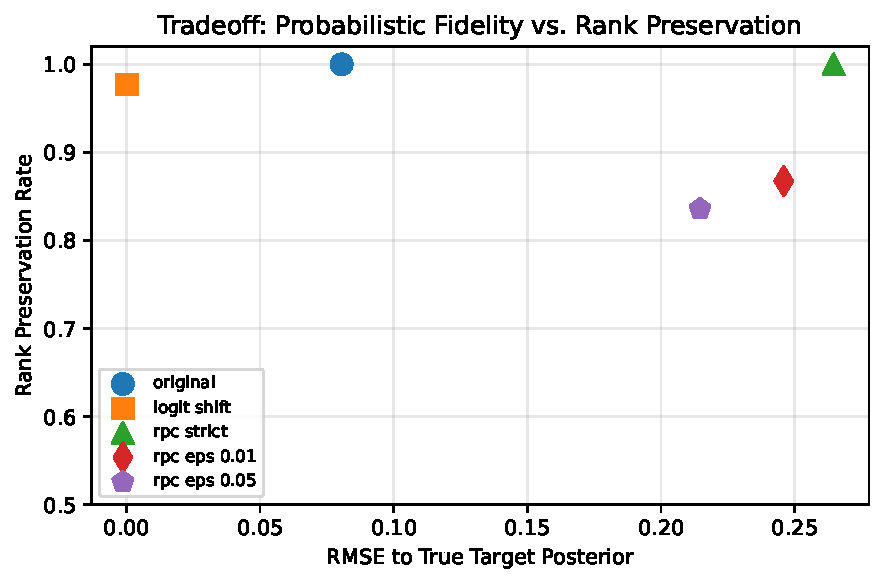
\includegraphics[width=0.8\textwidth]{experiments/output/synthetic_tradeoff.pdf}
\caption{Synthetic tradeoff: RMSE to true target posterior vs.\ rank preservation rate. Logit-shift achieves near-zero RMSE but scrambles ranks; strict RPC preserves ranks exactly but deviates from the true posterior; $\epsilon$-slack variants interpolate.}
\label{fig:synthetic}
\end{figure}

\subsection{Real-Data Shifted Deployment}
\label{sec:realdata}

We train 300-tree random forests \citep{pedregosa2011} on UCI \texttt{digits} and \texttt{wine} datasets, then create shifted holdout sets by resampling with altered class composition. We use exact target counts as $T$ and average over 5 random seeds.

\begin{table}[t]
\centering
\small
\caption{Real-data experiments with shifted class distributions. Results averaged over 5 random seeds. RPC-strict achieves exact column totals and rank preservation where it converges; on \texttt{digits} (10 classes with extreme shift), strict convergence fails and practitioners should use the nearly-isotonic variant.}
\label{tab:realdata}
\begin{tabular}{llcccc}
\toprule
Dataset & Method & Brier $\downarrow$ & ECE $\downarrow$ & Rank Rate $\uparrow$ & Col Err $\downarrow$ \\
\midrule
digits & logit\_shift & 0.156$\pm$0.036 & 0.134$\pm$0.038 & 0.922$\pm$0.020 & 49.18$\pm$16.54 \\
digits & original & 0.125$\pm$0.021 & 0.221$\pm$0.027 & 1.000$\pm$0.000 & 89.62$\pm$24.99 \\
digits & rpc\_eps\_0.02 & 0.254$\pm$0.099 & 0.236$\pm$0.050 & 0.770$\pm$0.022 & 0.00$\pm$0.00 \\
digits & rpc\_strict & --- & --- & --- & --- \\
\midrule
wine & logit\_shift & 0.051$\pm$0.046 & 0.064$\pm$0.048 & 0.977$\pm$0.013 & 3.14$\pm$2.30 \\
wine & original & 0.049$\pm$0.013 & 0.121$\pm$0.025 & 1.000$\pm$0.000 & 6.64$\pm$2.62 \\
wine & rpc\_eps\_0.02 & 0.097$\pm$0.083 & 0.082$\pm$0.057 & 0.860$\pm$0.057 & 0.00$\pm$0.00 \\
wine & rpc\_strict & 0.101$\pm$0.087 & 0.079$\pm$0.052 & 1.000$\pm$0.000 & 0.00$\pm$0.00 \\
\bottomrule
\end{tabular}
\end{table}


Figure~\ref{fig:real} shows the Brier-rank tradeoff across methods. Original probabilities preserve ranks by construction but fail to match target totals. Logit-shift achieves the best Brier score but breaks ranks and falls short of exact total matching (column error $>0$). RPC methods achieve exact total matching (column error $=0$), with RPC-strict additionally preserving ranks exactly where it converges.

\begin{figure}[t]
\centering
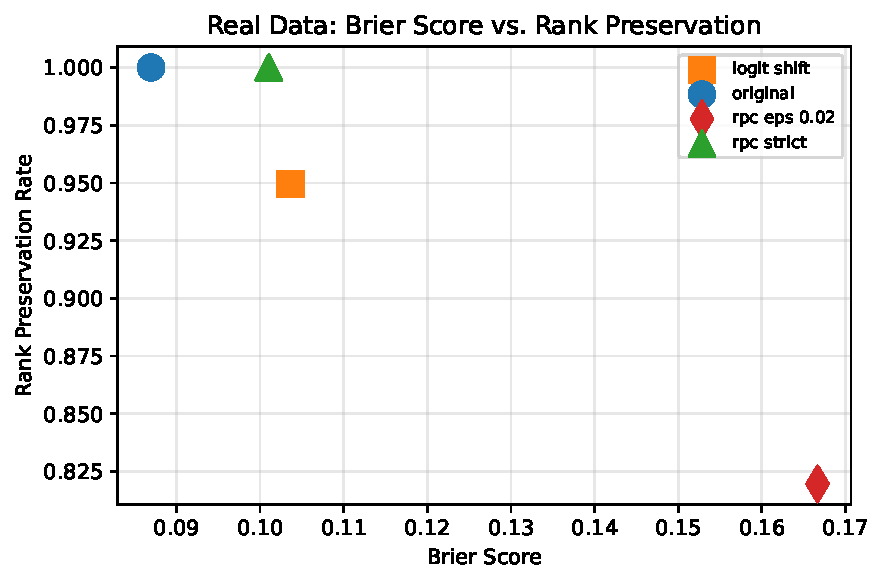
\includegraphics[width=0.8\textwidth]{experiments/output/brier_vs_rank.pdf}
\caption{Real data: Brier score vs.\ rank preservation rate across methods, averaged across both datasets and all seeds.}
\label{fig:real}
\end{figure}

\section{Discussion and Limitations}

The approach is suitable when relative ordering matters, as in regulatory triage, survey weighting, or fairness-constrained ranking. It is less suitable when the base model has poor discrimination (no meaningful ranks to preserve) or when computational budgets prohibit iterative projections on very large $N$, where stochastic variants may help.

The choice between methods depends on the downstream use. When predictions will be used to rank instances within classes, as in prioritization queues or risk rankings, preserving ranks is essential, and strict RPC is appropriate. When small rank violations are acceptable, the $\epsilon$-slack variants offer a smooth tradeoff, with $\epsilon$ tunable against a validation objective (Brier, ECE) or a domain-specific maximum tolerable violation. When the application cares only about expected loss minimization and not about individual instance comparisons, classical multiplicative reweighting (logit-shift) remains the right tool, with the understanding that ranks may not be preserved.

\section{Conclusion}
We presented a projection-based multiclass calibrator that preserves within-class rankings while matching population totals. The method reduces to PAV plus a scalar shift inside Dykstra or ADMM, is efficient in practice, and integrates into existing calibration pipelines.

\bibliographystyle{plainnat}
\bibliography{multiclass}

\end{document}
